\documentclass[12pt]{article}

% Packages for better typography and formatting
\usepackage{geometry}
\geometry{a4paper, margin=1in}
\usepackage{amsmath, amssymb}
\usepackage{graphicx}
\usepackage{hyperref}
\usepackage{cite}

\title{Title of the Scientific Report}
\author{Your Name \\
        Your Institution \\
        \texttt{your.email@domain.com}}
\date{\today}

\begin{document}

\maketitle

\begin{abstract}
    This is a brief summary of the report, highlighting the main objectives, methods, results, and conclusions. The abstract should provide a concise overview of the content and key findings.
\end{abstract}

\section{Introduction}
    The introduction should provide background information on the topic, outline the objectives of the report, and explain the significance of the work. Clearly state the problem or question addressed and summarize relevant previous research.

\section{Methods}
    Describe the experimental or computational methods used to obtain the results. Include details on materials, procedures, and any analytical techniques employed. Ensure that this section is detailed enough for replication of the work.

\section{Results}
    Present the main findings of your work. Use text, tables, and figures to clearly communicate the results. Figures should be accompanied by descriptive captions.

    \begin{figure}[h!]
        \centering
        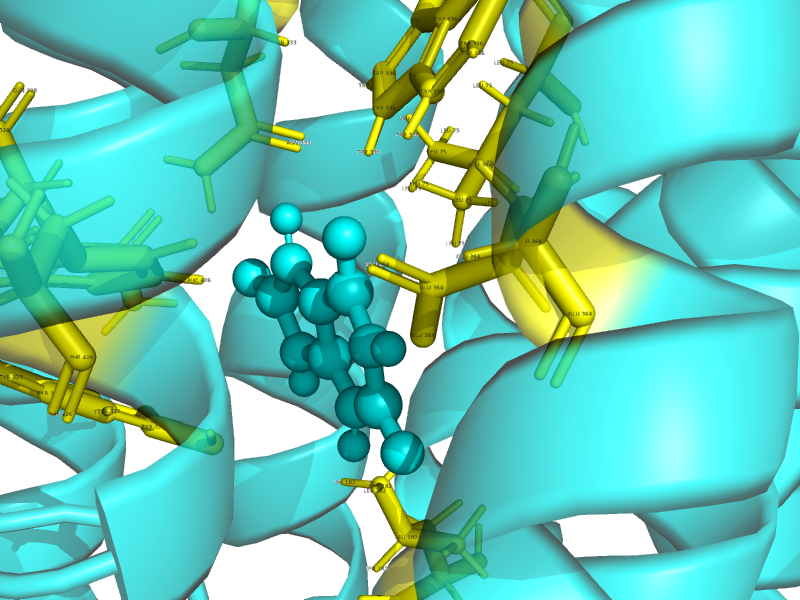
\includegraphics[width=0.7\textwidth]{./figures/membrane_protein.png}
        \caption{Caption for the figure.}
        \label{fig:example}
    \end{figure}

    \begin{table}[h!]
        \centering
        \begin{tabular}{|c|c|}
            \hline
            \textbf{Parameter} & \textbf{Value} \\
            \hline
            Example 1 & 10 \\
            Example 2 & 20 \\
            \hline
        \end{tabular}
        \caption{Caption for the table.}
        \label{tab:example}
    \end{table}

\section{Discussion}
    Interpret the results in the context of the objectives and previous research. Discuss any implications, limitations, and potential for future work. Compare your findings with those of other studies and explain any discrepancies.

\section{Conclusion}
    Summarize the key findings of the report and their significance. State any conclusions drawn from the results and their relevance to the field.

\section{References}
    Use the `\cite{}` command to reference the literature. Ensure that all references are properly cited and listed in the bibliography.

    \begin{thebibliography}{99}
        \bibitem{reference1} Author Name, \textit{Title of the Paper}, Journal Name, Volume (Year), Pages.
        \bibitem{reference2} Author Name, \textit{Title of the Book}, Publisher, Year.
    \end{thebibliography}

\end{document}